\documentclass[a4paper,12pt]{article}[abntex2]
\bibliographystyle{abntex2-alf}
\usepackage[table,xcdraw]{xcolor}

% Definições de layout e formatação
\usepackage[a4paper, left=3.0cm, top=3.0cm, bottom=2.0cm, right=2.0cm]{geometry} % Personalização das margens do documento
\usepackage{setspace} % Controle do espaçamento entre linhas
\onehalfspacing % Espaçamento entre linhas de 1,5
\usepackage{indentfirst} % Indentação do primeiro parágrafo das seções
\usepackage{newtxtext} % Substitui a fonte padrão pela Times Roman
\usepackage{titlesec} % Personalização dos títulos de seções
\usepackage{ragged2e} % Melhor controle de justificação do texto
\usepackage[portuguese]{babel} % Adaptação para o português (nomes e hifenização)
\usepackage{amsmath}

% Pacotes de cabeçalho, rodapé e títulos
\usepackage{fancyhdr} % Customização de cabeçalhos e rodapés
\setlength{\headheight}{14.49998pt} % Altura do cabeçalho
\pagestyle{fancy}
\fancyhf{} % Limpa cabeçalho e rodapé
\rhead{\thepage} % Página no canto direito do cabeçalho

% Pacotes para tabelas
\usepackage{booktabs} % Melhora a qualidade das tabelas
\usepackage{tabularx} % Permite tabelas com larguras de colunas ajustáveis
\usepackage{float} % Melhor controle sobre o posicionamento de figuras e tabelas

% Pacotes para gráficos e imagens
\usepackage{graphicx} % Suporte para inclusão de imagens

\usepackage[utf8]{inputenc}
\usepackage{listingsutf8}

\lstset{
    language=R,                      
    basicstyle=\ttfamily\scalefont{1.0},
    keywordstyle=\color{blue},       
    stringstyle=\color{red},         
    commentstyle=\color{green},      
    numbers=left,                    
    numberstyle=\tiny\color{gray},   
    stepnumber=1,                    
    numbersep=5pt,                   
    backgroundcolor=\color{lightgray!10}, 
    frame=single,                    
    breaklines=true,                 
    captionpos=b,                    
    keepspaces=true,                 
    showspaces=false,                
    showstringspaces=false,          
    showtabs=false,                  
    tabsize=2,
     literate={á}{{\'a}}1
             {é}{{\'e}}1
             {í}{{\'i}}1
             {ó}{{\'o}}1
             {ú}{{\'u}}1
             {Ú}{{\'U}}1
             {â}{{\^a}}1
             {ê}{{\^e}}1
             {î}{{\^i}}1
             {ô}{{\^o}}1
             {û}{{\^u}}1
             {ã}{{\~a}}1
             {õ}{{\~o}}1
             {ç}{{\c{c}}}1,
}


% Pacotes para unidades e formatação numérica
\usepackage{siunitx} % Tipografia de unidades do Sistema Internacional e formatação de números
\sisetup{
  output-decimal-marker = {,},
  inter-unit-product = \ensuremath{{}\cdot{}},
  per-mode = symbol
}
\DeclareSIUnit{\real}{R\$}
\newcommand{\real}[1]{R\$#1}

% Pacotes para hiperlinks e referências
\usepackage{hyperref} % Suporte a hiperlinks
\usepackage{footnotehyper} % Notas de rodapé clicáveis em combinação com hyperref
\hypersetup{
    colorlinks=true,
    linkcolor=black,
    filecolor=magenta,      
    urlcolor=cyan,
    citecolor=black,        
    pdfborder={0 0 0},
}
\makeatletter
\def\@pdfborder{0 0 0} % Remove a borda dos links
\def\@pdfborderstyle{/S/U/W 1} % Estilo da borda dos links
\makeatother

% Pacotes para texto e outros
\usepackage{lipsum} % Geração de texto dummy 'Lorem Ipsum'
\usepackage[normalem]{ulem} % Permite o uso de diferentes tipos de sublinhados sem alterar o \emph{}

\begin{document}

\begin{titlepage}
    \centering
    \vspace*{1cm}
    \Large\textbf{INSPER – INSTITUTO DE ENSINO E PESQUISA}\\
    \Large ECONOMIA\\
    \vspace{1.5cm}
    \Large\textbf{Atividade Prática Supervisionada - APS}\\
    \textbf{Comércio Internacional}\\
    \vspace{1.5cm}
    Prof. Arthur Augusto Viaro\\
    \vfill
    \normalsize
    Érika Kaori Fuzisaka, \href{mailto:erikakf1@al.insper.edu.br}{erikakf1@al.insper.edu.br}\\
    Hicham Munir Tayfour, \href{mailto:hichamt@al.insper.edu.br}{hichamt@al.insper.edu.br}\\

    \vfill
    São Paulo\\
    Abril/2025
\end{titlepage}

\newpage
\tableofcontents
\thispagestyle{empty} % Esse comando remove a numeração de pagina da tabela de conteúdo

\newpage 
\listoffigures
\thispagestyle{empty} % Esse comando remove a numeração de pagina da tabela de figura

\newpage
\listoftables
\thispagestyle{empty} % Este comando remove a numeração de página da lista de tabelas

\newpage
\setcounter{page}{1} % Inicia a contagem de páginas a partir desta página
\justify
\onehalfspacing

\section*{\textbf{Cenário Atual}} % Era para ser babado internacional
\addcontentsline{toc}{section}{Cenário Atual}

Nas últimas semanas, a decisão do governo dos EUA de implementar tarifas comerciais recíprocas sobre produtos de mais de 180 países, com alíquotas variando entre 10\% e 50\%, reacendeu o debate global sobre os impactos do protecionismo no comércio internacional. Em um cenário de crescente interdependência econômica, essa medida levanta importantes questionamentos sobre seus efeitos potenciais nos consumidores, produtores, trabalhadores e na dinâmica política e econômica tanto nos EUA quanto no restante do mundo. Este memorando tem como objetivo analisar as possíveis consequências dessa política tarifária, com base em teorias econômicas consolidadas e evidências empíricas, a fim de informar o público geral e contribuir para um debate sobre o tema.

\section*{\textbf{Impacto sobre consumidores}}
\addcontentsline{toc}{section}{Impacto sobre consumidores}

\subsection*{\textbf{EUA}}
\addcontentsline{toc}{subsection}{EUA}

Sob o \textbf{modelo ricardiano}, as tarifas elevam o preço interno dos bens importados; a linha orçamentária se torna mais horizontal, reduzindo o conjunto de cestas acessíveis e, portanto, o bem-estar. A Figura~\ref{fig:budget} ilustra essa rotação. Essa rotação transforma parte da renda do consumidor em receita de imposto e gera perda líquida de bem-estar. 

\begin{figure}[h]
  \centering
  \caption{Rotação da restrição orçamentária dos consumidores dos EUA após tarifa.}
  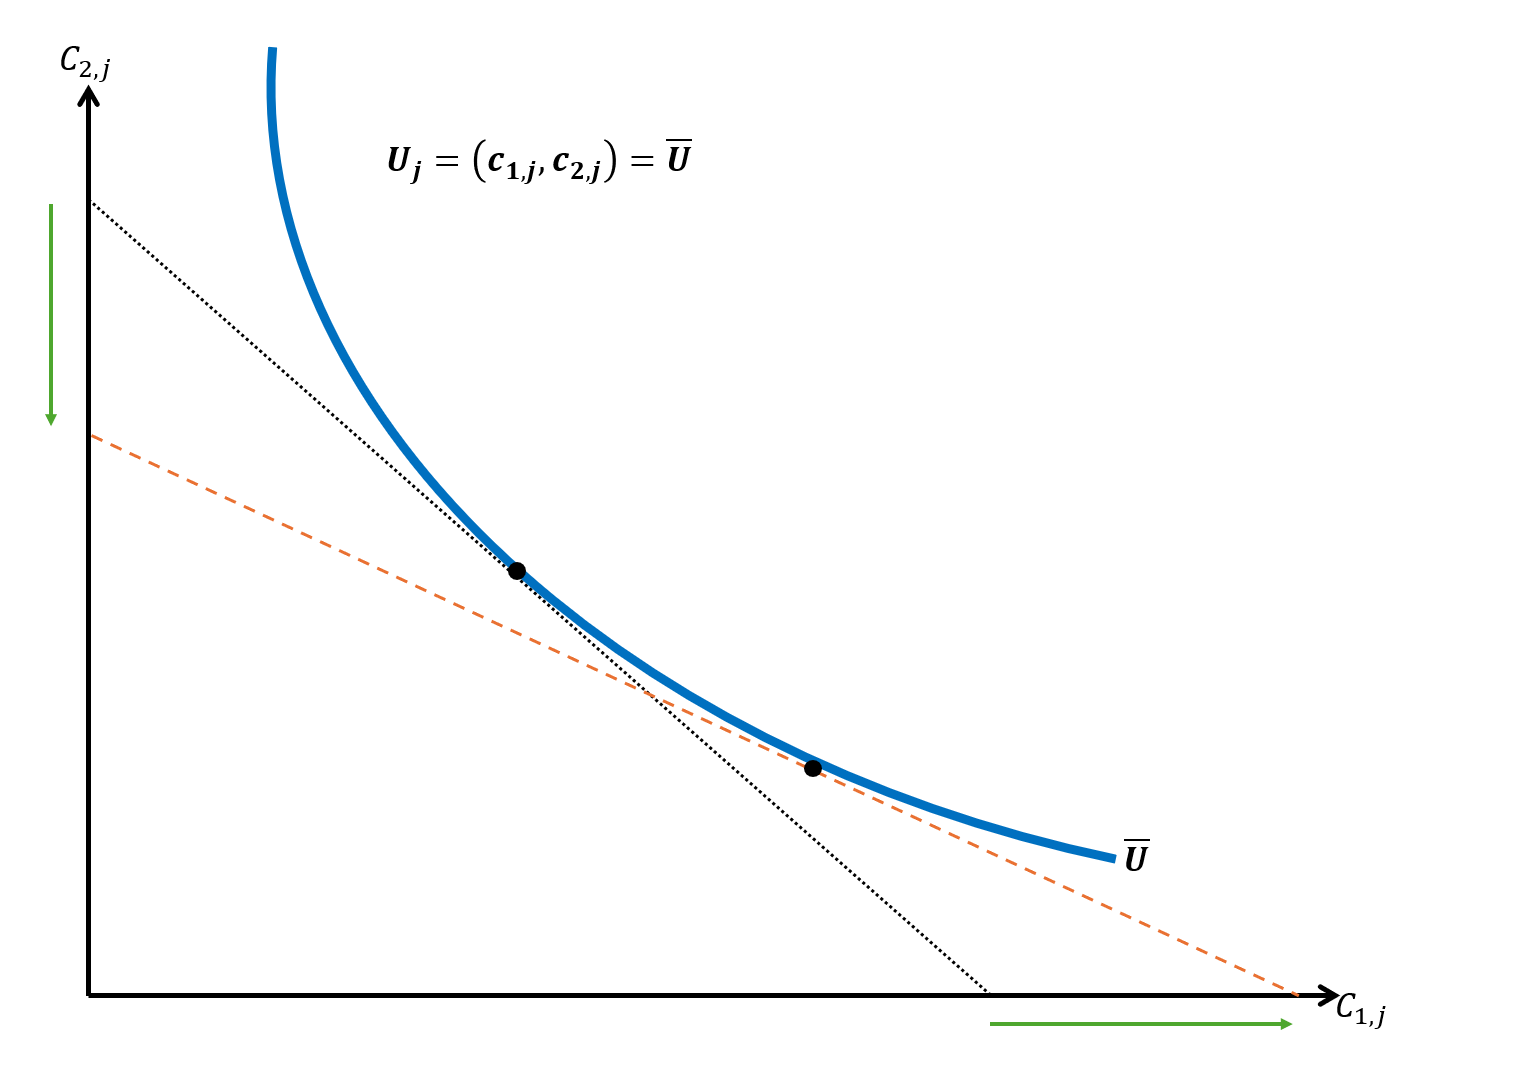
\includegraphics[width=0.7\linewidth]{Imagens/aps1i1.png}
  \label{fig:budget}
\end{figure}

Pela lógica de \textbf{Krugman (economias de escala e competição monopolística)}, quando a tarifa encarece o acesso ao mercado, parte das firmas estrangeiras sai dos EUA; cai o número de variedades disponíveis ($n\downarrow$). Com menos concorrência, as empresas que ficam aumentam sua margem de lucro, comprimindo ainda mais o excedente do consumidor (\emph{love for variety}).

\[
p_i' = (1+\tau) p_i
\]

No curtíssimo prazo não há substitutos domésticos suficientes; consumidores simplesmente pagam mais.  Com o tempo, fabricantes locais podem expandir a oferta, mas a literatura empírica mostra que a queda de preços raramente compensa totalmente a perda inicial de bem-estar.


\subsection*{\textbf{Resto do Mundo}}
\addcontentsline{toc}{subsection}{Resto do Mundo}

\begin{enumerate}
    \item \textbf{Em países afetados diretamente pelas tarifas}\\
   O desvio de demanda dos EUA cria excedente interno, pressionando o preço doméstico desses países \emph{para baixo}.  
   Para o consumidor local, isso significa pagar menos pelo menos no curto prazo. O mecanismo é o mesmo descrito no modelo Heckscher-Ohlin: um choque negativo no preço relativo do bem exportado se traduz em queda de preço interno e ganho imediato de excedente para quem compra.

    \item \textbf{Em países não-alvo, mas que podem abastecer o mercado norte-americano}\\
    O efeito é mais tênue. Alguns produtores desviam vendas para atender o mercado interno dos EUA, reduzindo a oferta interna, portanto eleva um pouco o preço local desses bens. Por outro lado, a pressão de baixa sobre o preço mundial de determinadas commodities também chega aos consumidores e pode contrabalançar esse movimento. Para o consumidor médio, o saldo costuma oscilar pouco, não uma alta generalizada. A teoria gravitacional de comércio sugere que o maior impacto nem é no preço, mas no custo logístico: tarifas e incerteza regulatória elevam frete e prazos, e parte disso é repassada ao varejo

    \item \textbf{No mundo todo (efeito de variedade e mark-up)}\\
    Mesmo onde os preços movem pouco, uma perda “silenciosa” é notada: menor variedade de produtos e margens maiores para produtos diferenciados. O modelo de economias de escala com concorrência monopolística (Krugman) mostra que, quando o maior mercado mundial encolhe, o número mundial de variedades viáveis diminui; com menos concorrência, as empresas restantes elevam seus mark-ups. Resultado: opções mais limitadas e aumentos em itens de nichos diferenciados (como vinhos, cosméticos, eletrônicos premium).
\end{enumerate}


\section*{\textbf{Impacto sobre os Produtores}}
\addcontentsline{toc}{section}{Impacto sobre os Produtores}


\subsection*{\textbf{Curto prazo}}
\addcontentsline{toc}{subsection}{Curto Prazo}

\begin{itemize}
  \item \textbf{EUA} – Nos setores explicitamente protegidos (como aço, alumínio), o preço de venda sobe assim que a tarifa entra em vigor. Com o capital ainda \emph{específico} ao setor, as margens aumentam rapidamente e parte desse ganho se reflete em salários setoriais maiores, como previsto no modelo de \textit{Fatores Específicos}. Já as firmas que dependem de insumos importados veem seus custos crescerem e perdem competitividade interna e externa.

  \item \textbf{Resto do mundo} – Exportadores que abasteciam o mercado estadunidense perdem pedidos quase imediatamente, gerando capacidade ociosa. O excedente é desviado para mercados domésticos ou terceiros países a preços menores, comprimindo margens. Concorrentes diretos dos EUA em mercados de terceiros podem ganhar volume, mas sob preços deprimidos.
\end{itemize}

\subsection*{\textbf{Longo prazo}}
\addcontentsline{toc}{subsection}{Longo prazo}

\begin{itemize}
  \item \textbf{EUA} – Com fatores de produção móveis, vale o Teorema de Rybczynski: insistir em bens intensivos em trabalho num país relativamente abundante em capital leva a uso ineficiente de recursos. A rentabilidade cai, parte do capital migra para setores não tarifados ou para o exterior, portanto a produtividade agregada recua. A proteção prolongada reduz incentivos à inovação; quando a concorrência externa diminui, o “bônus” inicial converge para zero à medida que cadeias globais se ajustam.
  \item \textbf{Resto do mundo} – As Firmas estrangeiras podem reagir de três maneiras: (i)instalam unidades nos EUA para contornar a tarifa, arcando com custos maiores; (ii)redirecionam vendas a novos mercados (América Latina, UE, Ásia); ou (iii)escalam na cadeia de valor, oferecendo bens diferenciados. Ainda assim, a contração do maior mercado mundial reduz a escala eficiente global e o número de variedades lucrativas, como o modelo de Krugman indica.
\end{itemize}

\section*{\textbf{Impacto sobre Trabalhadores}}
\addcontentsline{toc}{section}{Impacto sobre Trabalho}

\subsection*{\textbf{EUA}}
\addcontentsline{toc}{subsection}{Trabalhadores nos EUA}

\begin{itemize}
  \item \textbf{Setores protegidos} –  No curto prazo, pós choque, aço, alumínio, têxteis e ramos semelhantes vendem mais no mercado doméstico. A receita cresce e as empresas buscam operários adicionais; salários nominais sobem porque capital e equipamentos não conseguem mudar de setor de um dia para o outro (mecanismo do modelo de Fatores Específicos).\\
  No médio prazo, Parte do ganho nominal é consumida pela inflação gerada pela própria tarifa. Ainda assim, esses trabalhadores preservam alguma vantagem, pois a demanda interna continua deslocada a favor dos bens protegidos.
  
  E a longo prazo, uma vez que capital e trabalho passam a circular entre setores, vigora a lógica Stolper-Samuelson: o bem trabalho-intensivo segue relativamente caro e o salário real do operário menos qualificado permanece acima do que estaria sem a tarifa. Porém, quando a proteção se torna crônica, a menor concorrência externa reduz investimentos em P\&D; no quadro de longo prazo descrito por Krugman, a menor variedade e os mark-ups mais altos derrubam o crescimento de produtividade, limitando avanços salariais futuros.
  
  \item \textbf{Demais setores} – No curto prazo,indústrias que dependem de insumos importados como montadoras e de eletrônicos. Para defender margens, congelam salários, suspendem horas extras ou demitem. O encarecimento dos bens de consumo eleva o custo de vida, de modo que o salário real cai para a maioria dos trabalhadores fora dos setores protegidos.\\
  No médio prazo,empresas afetadas tentam redesenhar cadeias de suprimento, automatizar processos ou mesmo transferir parte da produção para o exterior. Empregos de qualificação intermediária encolhem; cresce a procura por profissionais de logística e de compras internacionais.
  No longo prazo, o retorno do capital fica menor e o salário dos qualificados avança menos do que avançaria num cenário de livre-comércio; toda a economia sente o freio no ganho de produtividade que decorre de menos variedade e menos escala.

\end{itemize}

\subsection*{\textbf{Resto do mundo}}
\addcontentsline{toc}{subsection}{Resto do mundo}

\begin{itemize}
  \item \textbf{Exportadores diretamente afetados} – Nos países que vendiam intensivamente para o mercado norte-americano, pedidos caem, turnos são reduzidos e salários nominais recuam nos setores atingidos.\\
  No médio prazo, Parte desses trabalhadores é realocada para vender em mercados alternativos, mas costuma receber salários menores; outras plantas fecham por falta de escala.
  E no longo prazo, a retração permanente do maior mercado consumidor faz a produtividade global crescer mais devagar; salários reais nesses países ficam abaixo da trajetória que seguiriam sem a tarifa.
  
  \item \textbf{Países terceiros que recebem desvio de comércio} – Em países que substituem parcialmente as vendas aos EUA, alguns ramos contratam mais e pagam salários um pouco maiores, mas o efeito é restrito a nichos específicos.\\
  No médio e longo prazos, quando a contração do mercado americano reduz o tamanho mínimo eficiente das cadeias globais, até esses ganhos pontuais desaparecem; o crescimento salarial desacelera de maneira generalizada, sobretudo em economias abundantes em mão-de-obra.
\end{itemize}

\section*{\textbf{Considerações Políticas}}
\addcontentsline{toc}{section}{Considerações Políticas}


\subsection*{\textbf{Grupos domésticos que tendem a apoiar}}
\addcontentsline{toc}{subsection}{Grupos domésticos que tendem a apoiar}

\begin{itemize}
    \item \textbf{Indústrias intensivas em trabalho pouco qualificado} (como siderurgia e metalurgia básica): concentram ganhos claros de curto prazo — preços de venda e retorno do capital específico aumentam.  
    \item \textbf{Sindicatos de setores protegidos}: veem a tarifa como mecanismo de preservar e elevar empregos na manufatura tradicional. 
    \item \textbf{Eleitores populistas/nacionalistas} que associam déficit comercial a perda de “grandeza” econômica ou segurança nacional.
\end{itemize}

\subsection*{\textbf{Grupos domésticos que tendem a se opor}}
\addcontentsline{toc}{subsection}{Grupos domésticos que tendem a se opor}

\begin{itemize}
    \item \textbf{Setores intensivos em importações} (automóveis, eletrônicos, construção): margens comprimem-se quando o custo de insumos estrangeiros sobe.  
    \item \textbf{Varejo de grande escala} e \textbf{empresas de e-commerce}: dependem de bens de consumo importados de baixo custo; repassem de preço atinge consumidores.  
    \item \textbf{Agronegócio e indústrias exportadoras}: temem retaliação estrangeira que feche mercados ou imponha quotas.  
    \item \textbf{Consumidores urbanos} e organismos pró-mercado que valorizam preços baixos e variedade; percebem o imposto oculto da tarifa.
\end{itemize}

\subsection*{\textbf{Possíveis repercussões internacionais}}
\addcontentsline{toc}{subsection}{Possíveis repercussões internacionais}


\begin{enumerate}
    \item \textbf{Retaliação tarifária} — parceiros afetados (UE, China, México, Canadá) podem impor tarifas equivalentes sobre exportações dos EUA, sobretudo em bens agrícolas e manufaturas politicamente sensíveis.  
    \item \textbf{Disputas na OMC} — países recorrerão ao mecanismo de solução de controvérsias; demora de anos aprofunda incerteza regulatória.  
    \item \textbf{Erosão da credibilidade multilateral} — a medida incentiva acordos regionais ou bilaterais que excluam os EUA, fortalecendo alianças comerciais alternativas (RCEP, UE e Mercosul).  
    \item \textbf{Escalada protecionista} — outros governos podem usar o precedente para justificar barreiras “recíprocas”, elevando o custo global de comércio e fragmentando cadeias de valor.  
    \item \textbf{Repercussões geopolíticas} — aliados tradicionais questionam o compromisso dos EUA com normas internacionais; rivais estratégicos (China) aproveitam o vácuo para projetar liderança em comércio e investimento.
\end{enumerate}


\section*{\textbf{Impacto Macroeconômico e Países Mais Afetados}}
\addcontentsline{toc}{section}{Impacto Macroeconômico e Países Mais Afetados}

\subsection*{\textbf{EUA}}
\addcontentsline{toc}{subsection}{EUA}


Do ponto de vista da teoria, as tarifas levam a economia norte-americana para fora da sua vantagem comparativa. Nos modelos referenciados, um país relativamente abundante em capital, como os EUA, torna-se menos eficiente quando passa a produzir bens mais intensivos em trabalho que antes importava. Essa realocação faz a fronteira de possibilidades de consumo recuar e reduz o bem-estar agregado. No curto prazo, o modelo de fatores específicos ajuda a entender por que os setores protegidos inicialmente prosperam: o preço doméstico dos seus produtos sobe enquanto o capital permanece preso ao setor, elevando lucros e salários locais. Entretanto, consumidores e indústrias que dependem de insumos importados enfrentam preços mais altos, de modo que o ganho concentrado desses ramos não compensa o “imposto” espalhado pelo resto da economia. Quando se consideram as economias de escala descritas por Krugman, a situação piora: a redução de importações diminui a variedade disponível, encolhe a escala ótima de produção e eleva as margens de monopólio, o que prejudica a produtividade total dos fatores. Em conjunto, esses mecanismos apontam para um leve recuo do PIB real, inflação de bens protegidos e queda na eficiência produtiva doméstica.

\subsection*{\textbf{Resto do mundo}}
\addcontentsline{toc}{subsection}{Resto do mundo}


No exterior, a lógica se inverte. Países abundantes em trabalho (tipicamente exportadores de bens intensivos nesse fator) perdem parte da demanda no item em que são mais eficientes, que deprime o preço relativo do produto e reduz salários reais. Com capital e trabalhadores específicos a esse setor, a queda de receita se traduz em cortes de emprego e deslocamento de mão de obra para atividades menos produtivas. Além disso, a contração do maior mercado consumidor do mundo reduz o número de variedades globalmente rentáveis, comprimindo a escala das plantas industriais e, por consequência, a produtividade mundial. O modelo de competição monopolística mostra que esse efeito de menor variedade gera perda de bem-estar mesmo para países que não são alvo direto das tarifas.

Os impactos distribuem-se de forma desigual entre os parceiros comerciais dos EUA. México e Canadá, altamente integrados às cadeias de valor norte-americanas, sofrem tanto na exportação de bens finais como na venda de componentes automotivos. Vietnã, Bangladesh e outros exportadores intensivos em mão-de-obra ressentem-se da queda imediata nas encomendas de têxteis e calçados. China e Coreia do Sul, grandes fornecedores de insumos eletrônicos, são afetadas duplamente: pelo encarecimento de seus produtos nos EUA e pela possível realocação das linhas de montagem que utilizam esses componentes. Pequenas economias muito abertas, como Singapura, Malásia ou Chile acabam sendo expostas a uma retração geral do comércio, vendo a sua atividade doméstica recuar de maneira desproporcional. Em síntese, as tarifas reduzem a eficiência dentro dos EUA, retiram renda dos exportadores mais dependentes do mercado norte-americano e, ao fragmentar as cadeias globais, impõem um custo de menor escala e menor produtividade da economia mundial.

\section*{\textbf{Conclusão}}
\addcontentsline{toc}{section}{Conclusão}
À luz das principais teorias de comércio internacional e da evidência empírica recente, as tarifas recíprocas \textbf{diminuem o bem‑estar agregado}, beneficiam grupos específicos às custas de consumidores e produtores integrados a cadeias globais, e alimentam retaliações que erodem a posição dos EUA no sistema multilateral. Políticas alternativas de apoio à competitividade ––qualificação de trabalhadores e inovação–—oferecem custo‑benefício superior sem comprometer os \textit{ganhos de troca} que sustentam o crescimento global.

\end{document}

\newpage
% Memorando de Política – Tarifas Recíprocas dos EUA
% Curso: Comércio Internacional – APS 2025S1
% Autor: <seu nome aqui>
% Data de submissão: 28 de abril de 2025

% ==========================
\section*{Resumo Executivo}
As ``tarifas recíprocas'' anunciadas pelos Estados Unidos––entre \(10\%\) e \(50\%\) para mais de 180 países––\textbf{encarecem bens importados, reduzem poder de compra dos consumidores e deslocam produção}. A literatura de comércio internacional indica que os \textit{ganhos de troca} provêm de preços mais baixos, especialização conforme \textit{vantagens comparativas} e acesso a maior variedade de produtos. As novas tarifas revertem parte desses ganhos, gerando:
\begin{itemize}
  \item perda de bem‐estar para consumidores norte‑americanos e estrangeiros;
  \item redistribuição de renda entre setores e fatores de produção (curto e longo prazos);
  \item tensões políticas internas e retaliações externas que potencialmente amplificam os custos econômicos.
\end{itemize}
Concluímos que a medida é, no agregado, \textbf{desfavorável ao bem‐estar mundial} e contraproducente aos objetivos declarados de fortalecimento industrial dos EUA.

% ==========================
\section{Impacto sobre Consumidores}
\subsection*{EUA}
Sob o \textbf{modelo ricardiano}, tarifas elevam o preço interno dos bens importados acima do custo marginal estrangeiro; a curva de orçamentos dos consumidores gira para dentro, reduzindo utilidade (Fig.~\ref{fig:budget}). Estimativas recentes indicam elasticidades de pass‑through superiores a \(0{,}9\), ou seja, o sobrepreço recai quase integralmente sobre o comprador final.

Pela lógica \textbf{Krugman (economias de escala e competição monopolística)}, consumidores também perdem variedade: menores mercados efetivos reduzem o número de variedades disponíveis, diminuindo o termo de amor pela diversidade \((n^{1-\gamma})\) na função CES.

\subsection*{Resto do mundo}
Exportadores atingidos enfrentam queda na demanda; parte do excedente é redirecionado a terceiros mercados a preços de liquidação, comprimindo margens globais. Para países pequenos, termos de troca se deterioram; para grandes players (UE, China), efeitos dependem da elasticidade da oferta doméstica e das contramedidas.

% ==========================
\section{Impacto sobre Produtores}
\subsection*{Curto prazo – Modelo de Fatores Específicos}
Bens protegidos (aço, alumínio, têxteis) veem seus preços relativos subir. Segundo o \textbf{modelo de fatores específicos}, o capital específico desses setores (máquinas, instalações) aufere renda extra \((\uparrow r_{setor})\), enquanto o capital nos setores exportadores (soja, aviões) sofre \((\downarrow r)\). A mobilidade limitada de capital e trabalho no horizonte de 1–2 anos amplifica ganhos e perdas.

\subsection*{Longo prazo – Heckscher–Ohlin}
Com mobilidade completa de fatores, retornos ao trabalho e ao capital tendem a equalizar‑se, mas \textbf{Stolper–Samuelson} prevê que \textit{o fator utilizado intensivamente no setor protegido} (trabalho pouco qualificado na manufatura tradicional) se beneficia relativamente, enquanto capital e trabalho qualificado perdem. Entretanto, após o ajuste: (i) insumos importados mais caros elevam custos; (ii) retaliação reduz demanda externa. Diversos estudos (Autor, Dorn, Hanson, 2013) mostram ganhos líquidos nulos em manufaturas americanas após tarifas sobre pneus chineses (2009).

% ==========================
\section{Impacto sobre Trabalhadores}
\begin{itemize}
  \item \textbf{Estados Unidos}: ganhos reais concentram‑se em grupos com alta parcela de renda proveniente de setores visados (siderurgia \& metalurgia). Trabalhadores de serviços, distribuídos por toda a economia, enfrentam preços de bens duráveis e alimentos mais altos, reduzindo salário real. Estudos de \textit{input–output} sugerem que cada vaga preservada em aço custa \~\$900 mil anuais ao consumidor.
  \item \textbf{Estrangeiro}: setores intensivos em trabalho (têxteis do Vietnã; calçados do Brasil) sofrem cortes de produção; salários caem via canal de demanda. Contudo, num cenário de retaliação, produtores agrícolas americanos podem ser substituídos por argentinos ou australianos, beneficiando seus trabalhadores.
\end{itemize}

% ==========================
\section{Considerações Políticas}
\subsection*{Grupos domésticos}
\begin{description}
  \item[Favorecidos:] Associações industriais dos setores protegidos; sindicatos da manufatura tradicional em Estados‑chave (Pensilvânia, Ohio). Ganhos são visíveis e concentrados.
  \item[Opositores:] Importadores, varejistas (Walmart), exportadores agrícolas (Midwest), firmas que dependem de insumos importados (indústria automotiva) e consumidores em geral. Perdas são dispersas, dificultando mobilização.
\end{description}

\subsection*{Reações internacionais}
OMC permite tarifas \textit{de retaliação equivalente}. Parceiros podem (e vêm sinalizando) sobretaxar soja, bourbon, motocicletas e produtos culturais, mirando redutos políticos americanos. Há risco de perder credibilidade na liderança do sistema multilateral, incentivando acordos regionais que excluam os EUA.

% ==========================
\section{Impacto Macroeconômico e Países Mais Afetados}
\subsection*{Estados Unidos}
Modelagens de equilíbrio geral (USITC, 2019) estimam que um choque tarifário médio de 20\% reduza PIB de longo prazo em até 0,5\% e destrua 150\,000 empregos líquidos, devido ao efeito cascata no custo de insumos e revide externo. Ganhos de receita tarifária (\$30–40 bi) são ofuscados pela queda de excedente do consumidor (\$80–100 bi).

\subsection*{Resto do mundo}
\begin{itemize}
  \item \textbf{México e Canadá}: elevada integração via USMCA; desvio de comércio significativo.
  \item \textbf{China}: alvo de escalada tarifária; perdas de curto prazo em eletrônicos, mas potencial substituição de fornecedores agrícolas.
  \item \textbf{União Europeia}: impacto moderado; possibilidade de liderança normativa.
  \item \textbf{Países em desenvolvimento exportadores de commodities}: oportunidades de ganhar participação nos EUA, mas exposição a desaceleração global.
\end{itemize}

% ==========================
\section{Conclusão}
À luz das principais teorias de comércio internacional e da evidência empírica recente, as tarifas recíprocas \textbf{diminuem o bem‑estar agregado}, beneficiam grupos específicos às custas de consumidores e produtores integrados a cadeias globais, e alimentam retaliações que erodem a posição dos EUA no sistema multilateral. Políticas alternativas de apoio à competitividade ––qualificação de trabalhadores e inovação–—oferecem custo‑benefício superior sem comprometer os \textit{ganhos de troca} que sustentam o crescimento global.  



% ==========================


